\subsection{Grammatical approach}

%#############################################################################################################%
%#############################################################################################################%

\begin{frame}[fragile]
  \frametitle{Dependency tree output by the Stanford Parser}

\begin{figure}
  \begin{tikzpicture}
    \node (0) at (10,10) {ROOT};
    \node (1) at (10,8.5) {live};
    \node (2) at (8,7) {minister};
    \node (3) at (10,7) {does};
    \node (4) at (12,7) {Where};
    \node (5) at (6,5.5) {the};
    \node (6) at (8,5.5) {prime};
    \node (7) at (10,5.5) {Kingdom};
    \node (8) at (11,4) {United};
    \node (9) at (9,4) {the};

    \node (10) at (14,1) {}; % utilisé pour forcer le positionnement de la figure globale

    \draw[->, >=latex] (0) edge node[anchor=center, right] {\scriptsize{root}} (1);
    \draw[->, >=latex] (1) edge node[anchor=center, left] {\scriptsize{nsubj}} (2);
    \draw[->, >=latex] (1) edge node[anchor=center, right] {\scriptsize{aux}} (3);
    \draw[->, >=latex] (1) edge node[anchor=center, right] {\scriptsize{advmod}} (4);
    \draw[->, >=latex] (2) edge node[anchor=center, left] {\scriptsize{det}} (5);
    \draw[->, >=latex] (2) edge node[anchor=center, right] {\scriptsize{prep\_of}} (7);
    \draw[->, >=latex] (2) edge node[anchor=center, left] {\scriptsize{amod}} (6);
    \draw[->, >=latex] (7) edge node[anchor=center, right] {\scriptsize{nn}} (8);
    \draw[->, >=latex] (7) edge node[anchor=center, left] {\scriptsize{det}} (9);
  \end{tikzpicture}
\end{figure}

\end{frame}

%#############################################################################################################%
%#############################################################################################################%

\begin{frame}[fragile]
  \frametitle{Identify question word}

\begin{figure}
  \begin{tikzpicture}
    \node (0) at (10,10) {ROOT};
    \node (1) at (10,8.5) {live};
    \node (2) at (8,7) {minister};
    \node (3) at (10,7) {does};
    \onslide<1>{\node (4) at (12,7) {Where};}
    \node (5) at (6,5.5) {the};
    \node (6) at (8,5.5) {prime};
    \node (7) at (10,5.5) {Kingdom};
    \node (8) at (11,4) {United};
    \node (11) at (9,4) {the};
  
    \node (9) at (14,1) {}; % utilisé pour forcer le positionnement de la figure globale

    \onslide<1>{\draw [draw=orange] (11.4,7.2) rectangle (12.6,6.8);}
    \onslide<1>{\node (10) at (13,6.5) {\footnotesize{Question word}};}
  
    \draw[->, >=latex] (0) edge node[anchor=center, right] {\scriptsize{root}} (1);
    \draw[->, >=latex] (1) edge node[anchor=center, left] {\scriptsize{nsubj}} (2);
    \draw[->, >=latex] (1) edge node[anchor=center, right] {\scriptsize{aux}} (3);
    \onslide<1>{\draw[->, >=latex] (1) edge node[anchor=center, right] {\scriptsize{advmod}} (4);}
    \draw[->, >=latex] (2) edge node[anchor=center, left] {\scriptsize{det}} (5);
    \draw[->, >=latex] (2) edge node[anchor=center, right] {\scriptsize{prep\_of}} (7);
    \draw[->, >=latex] (2) edge node[anchor=center, left] {\scriptsize{amod}} (6);
    \draw[->, >=latex] (7) edge node[anchor=center, right] {\scriptsize{nn}} (8);
    \draw[->, >=latex] (7) edge node[anchor=center, left] {\scriptsize{det}} (11);
  
    \onslide<2->{}
  \end{tikzpicture}
\end{figure}
  
\end{frame}

%#############################################################################################################%
%#############################################################################################################%

\begin{frame}[fragile]
  \frametitle{Merging}

\begin{figure}
 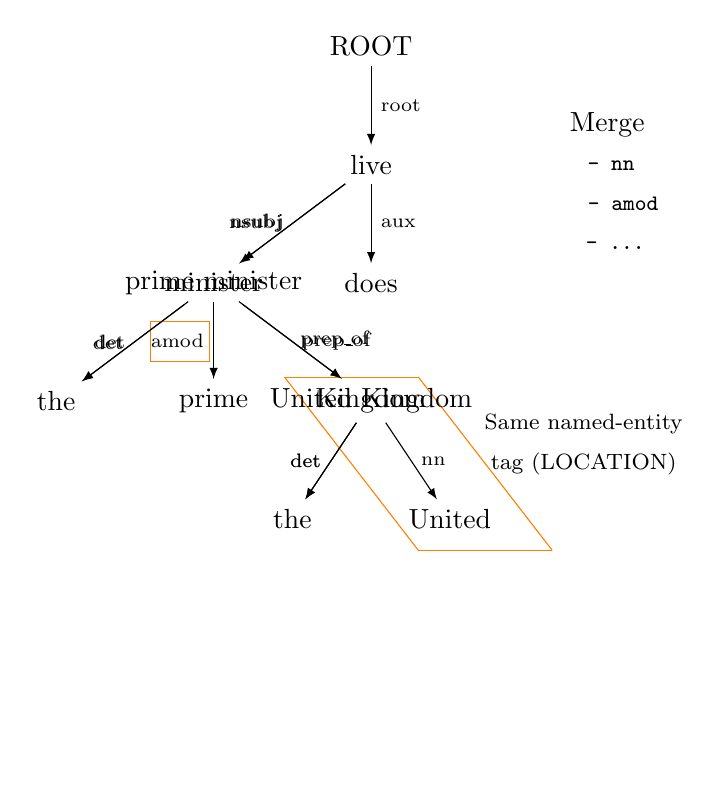
\begin{tikzpicture}
  \node (0) at (10,10) {ROOT};
  \node (1) at (10,8.5) {live};
  \onslide<-3>{\node (2) at (8,7) {minister};}
  \node (3) at (10,7) {does};
  \node (5) at (6,5.5) {the};
  \onslide<-3>{\node (6) at (8,5.5) {prime};}
  \onslide<1>{\node (7) at (10,5.5) {Kingdom};}
  \onslide<1>{\node (8) at (11,4) {United};}
  \node (13) at (9,4) {the};

  \node (9) at (14,1) {}; % utilisé pour forcer le positionnement de la figure globale

  \onslide<1>{\draw [draw=orange] (8.9,5.8) -- (10.6,3.6);}
  \onslide<1>{\draw [draw=orange] (10.6,5.8) -- (12.3,3.6);}
  \onslide<1>{\draw [draw=orange] (8.9,5.8) -- (10.6,5.8);}
  \onslide<1>{\draw [draw=orange] (10.6,3.6) -- (12.3,3.6);}
  \onslide<1>{\node (10) at (12.7,5.2) {\footnotesize{Same named-entity}};}
  \onslide<1>{\node (11) at (12.7,4.7) {\footnotesize{tag (\alert{LOCATION})}};}

  \onslide<2->{\node (12) at (10,5.5) {United Kingdom};}

  \draw[->, >=latex] (0) edge node[anchor=center, right] {\scriptsize{root}} (1);
  \onslide<-3>{\draw[->, >=latex] (1) edge node[anchor=center, left] {\scriptsize{nsubj}} (2);}
  \draw[->, >=latex] (1) edge node[anchor=center, right] {\scriptsize{aux}} (3);
  \onslide<-3>{\draw[->, >=latex] (2) edge node[anchor=center, left] {\scriptsize{det}} (5);}
  \onslide<-3>{\draw[->, >=latex] (2) edge node[anchor=center, right] {\scriptsize{prep\_of}} (7);}
  \onslide<-3>{\draw[->, >=latex] (2) edge node[anchor=center, left] {\scriptsize{amod}} (6);}
  \onslide<1>{\draw[->, >=latex] (7) edge node[anchor=center, right] {\scriptsize{nn}} (8);}
  \onslide<-2>{\draw[->, >=latex] (7) edge node[anchor=center, left] {\scriptsize{det}} (13);}
  \onslide<3->{\draw[->, >=latex] (12) edge node[anchor=center, left] {\scriptsize{det}} (13);}
  
  % fusion du amod
  
  \onslide<3>{\draw [draw=orange] (7.2,6.5) rectangle (7.95,6);}
  
  \onslide<3,4>{
  \node (13) at (13,9) {\alert{Merge}};
  \node (14) at (13.05,8.5) {\footnotesize{\texttt{- nn}}}; 
  \node (15) at (13.2,8) {\footnotesize{\texttt{- amod}}}; 
  \node (16) at (13.1,7.5) {\footnotesize{\texttt{- ...}}};}

  \onslide<4->{\node (17) at (8,7) {prime minister};}
  \onslide<4>{\draw[->, >=latex] (1) edge node[anchor=center, left] {\scriptsize{nsubj}} (17);}
  \onslide<4>{\draw[->, >=latex] (17) edge node[anchor=center, right] {\scriptsize{prep\_of}} (7);}
  \onslide<4>{\draw[->, >=latex] (17) edge node[anchor=center, left] {\scriptsize{det}} (5);}
  \end{tikzpicture}
\end{figure}
  
\end{frame}

%#############################################################################################################%
%#############################################################################################################%

\begin{frame}[fragile]
  \frametitle{Removal}

\begin{figure}
 \begin{tikzpicture}
  \node (0) at (10,10) {ROOT};
  \node (1) at (10,8.5) {live};
  \node (2) at (8,7) {prime minister};
  \onslide<1>{\node (3) at (10,7) {does};}
  \onslide<1>{\node (5) at (6,5.5) {the};}
  \node (7) at (10,5.5) {United Kingdom};
  \onslide<1>{\node (13) at (9,4) {the};}

  \node (8) at (14,1) {}; % utilisé pour forcer le positionnement de la figure globale

  \onslide<1>{\draw [draw=orange] (6.4,6.5) rectangle (7,5.9);}
  \onslide<1>{\draw [draw=orange] (10.05,7.9) rectangle (10.6,7.6);}
  \onslide<1>{\draw [draw=orange] (8.9,4.95) rectangle (9.5,4.5);}
  
  \node (9) at (13,9) {\alert{Remove}};
  \node (10) at (13.1,8.5) {\footnotesize{\texttt{- det}}}; 
  \node (11) at (13.1,8) {\footnotesize{\texttt{- aux}}}; 
  \node (12) at (13.1,7.5) {\footnotesize{\texttt{- ...}}};
  
  \draw[->, >=latex] (0) edge node[anchor=center, right] {\scriptsize{root}} (1);
  \draw[->, >=latex] (1) edge node[anchor=center, left] {\scriptsize{nsubj}} (2);
  \onslide<1>{\draw[->, >=latex] (1) edge node[anchor=center, right] {\scriptsize{aux}} (3);}
  \onslide<1>{\draw[->, >=latex] (2) edge node[anchor=center, left] {\scriptsize{det}} (5);}
  \draw[->, >=latex] (2) edge node[anchor=center, right] {\scriptsize{prep\_of}} (7);
  \onslide<1>{\draw[->, >=latex] (7) edge node[anchor=center, left] {\scriptsize{det}} (13);}

  \onslide<2>{} % forcer slide 2
  \end{tikzpicture}
\end{figure}
  
\end{frame}

%#############################################################################################################%
%#############################################################################################################%

\begin{frame}[fragile]
  \frametitle{Nounification}

\begin{figure}
 \begin{tikzpicture}
  \node (0) at (10,10) {ROOT};
  \onslide<1>{\node (1) at (10,8.5) {live};}
  \node (2) at (8,7) {prime minister};
  \node (7) at (10,5.5) {United Kingdom};

  \node (8) at (6.45,1) {}; % utilisé pour forcer le positionnement de la figure globale

  \onslide<1>{\draw[->, >=latex] (0) edge node[anchor=center, right] {\scriptsize{root}} (1);}
  \onslide<1>{\draw[->, >=latex] (1) edge node[anchor=center, left] {\scriptsize{nsubj}} (2);}
  \draw[->, >=latex] (2) edge node[anchor=center, right] {\scriptsize{prep\_of}} (7);
  
  \node (18) at (12.7,9) {\alert{Nounify}};
  \onslide<1>{\draw [draw=mLightBrown] (9.6,8.7) rectangle (10.4,8.3);}
  
  \onslide<2->{\node (22) at (10,8.5) {residence};}
  \onslide<2->{\draw[->, >=latex] (0) edge node[anchor=center, right] {\scriptsize{root}} (22);}
  \onslide<2->{\draw[->, >=latex] (22) edge node[anchor=center, left] {\scriptsize{nsubj}} (2);}
  \end{tikzpicture}
\end{figure}
  
\end{frame}

%#############################################################################################################%
%#############################################################################################################%

\begin{frame}[fragile]
  \frametitle{Normalization}
  
\begin{figure}
 \begin{tikzpicture}
  \node (0) at (9,10) {ROOT};
  \node (1) at (9,8.5) {residence};
  \node (2) at (9,7) {prime minister};
  \node (3) at (9,5.5) {United Kingdom};

  \draw[->, >=latex] (0) edge node[anchor=center, right] {\scriptsize{root}} (1);
  \draw[->, >=latex] (1) edge node[anchor=center, right] {\scriptsize{nsubj}} (2);
  \draw[->, >=latex] (2) edge node[anchor=center, right] {\scriptsize{prep\_of}} (3); 

  \onslide<1-2>{\draw [draw=mLightBrown] (15,10) rectangle (16.5,9);}
  \onslide<1-2>{\node (20) at (15,9.5) {};}
  \onslide<1>{\node (21) at (10.5,9.5) {};}
  \onslide<2>{\node (22) at (10.5,8.5) {};}
  \onslide<3>{\node (23) at (10.5,6) {};}
  \onslide<3>{\node (24) at (14.3,8) {};}
  \onslide<4>{\node (25) at (10.5,5.75) {};}
  \onslide<4>{\node (26) at (12.3,6.75) {};}
  
  \onslide<1>{\draw[->, >=latex] [draw=mLightBrown] (21) edge node[anchor=center, right, above] {\scriptsize{\produ}} (20);}
  \onslide<2>{\draw[->, >=latex] [draw=mLightBrown] (22) edge node[anchor=center, sloped, right, above] {\scriptsize{\produ}} (20);}
  \onslide<3>{\draw[->, >=latex] [draw=mLightBrown] (23) edge node[anchor=center, sloped, right, above] {\scriptsize{\produ}} (24);}
  \onslide<4>{\draw[->, >=latex] [draw=mLightBrown] (25) edge node[anchor=center, sloped, right, above] {\scriptsize{\produ}} (26);}

  \onslide<1>{\draw [draw=mLightBrown] (7.5,10.5) rectangle (10.5,5);}
  \onslide<2>{\draw [draw=mLightBrown] (7.5,9) rectangle (10.5,5);}
  \onslide<3>{\draw [draw=mLightBrown] (7.5,7.5) rectangle (10.5,5);}
  \onslide<4>{\draw [draw=mLightBrown] (7.5,6) rectangle (10.5,5);}

  %%%%
  
  \onslide<3->{
  \node (4) at (16.5,10) {$\triple$};
  \node (5) at (14.6,8.5) {};
  \node (6) at (16.5,8.5) {residence};
  \node (7) at (18.2,8.5) {?};

  \draw[->, >=latex] (4) edge node[sloped, anchor=center, above] {\scriptsize{pred.}} (6);
  \draw[->, >=latex] (4) edge node[sloped, anchor=center, above] {\scriptsize{obj.}} (7); }
  \onslide<3>{\draw[->, >=latex] (4) edge node[sloped, anchor=center, above] {\scriptsize{subj.}} (5);}
  
  \onslide<3>{\draw [draw=mLightBrown] (14.3,8.5) rectangle (15.2,7.8);}

  \onslide<4->{
  \node (8) at (14.5,8.5) {$\triple$};
  \node (9) at (12.5,7) {};
  \node (10) at (14.5,7) {prime minister};
  \node (11) at (16.5,7) {?};

  \draw[->, >=latex] (4) edge node[sloped, anchor=center, above] {\scriptsize{subj.}} (8);
  \draw[->, >=latex] (8) edge node[sloped, anchor=center, above] {\scriptsize{pred.}} (10);
  \draw[->, >=latex] (8) edge node[sloped, anchor=center, above] {\scriptsize{obj.}} (11); }

  \onslide<4>{\draw[->, >=latex] (8) edge node[sloped, anchor=center, above] {\scriptsize{subj.}} (9);}

  \onslide<4>{\draw [draw=mLightBrown] (12.3,7) rectangle (13,6.5);}
  
  \onslide<5>{\node (12) at (11.8,7) {United Kingdom};
  \draw[->, >=latex] (8) edge node[sloped, anchor=center, above] {\scriptsize{subj.}} (12);}
 \end{tikzpicture}
\end{figure}

\end{frame}